\section{Using Project-Join Trees for Projected Model Counting}
In this section, we adapt the framework from Chapter \ref{ch:dpmc} in order to perform projected model counting. 
Recall that Chapter \ref{ch:dpmc} describes a two-phase algorithm for computing the weighted model count of a CNF formula $\phi$. First, the \emph{planning phase} in Section \ref{sec_planning} builds a project-join tree $(T, r, \gamma, \pi)$ of $\phi$.
Second, the \emph{execution phase} in Section \ref{sec_execution} computes the $W$-valuation of the project-join tree to obtain the weighted model count.

In order to adapt this framework to perform weighted projected model counting, we aim to modify the valuation of project-join trees to incorporate both disjunctive variables and additive variables. In particular, we must perform $\exists$-projection with all disjunctive variables and $\Sigma$-projection with all additive variables.

% In \cite{dudek2020dpmc}, performing this traversal on \emph{every} project-join tree for a CNF formula $\phi$ produces the same result: the weighted model count of $\phi$. This stems from the fact that, for weighted model counting, all projections are $\Sigma$-projections and so all projections commute. There is therefore no restriction on the order that variables can appear in the project-join tree.

The challenge is that not all projections commute: $\Sigma$-projections do not commute with $\exists$-projections in general. Since the $\exists$-projections appear on the inside of the expression for projected model counting, we must ensure that all $\exists$-projections occur before all $\Sigma$-projections while traversing the project-join tree. We formalize this by requiring the project-join tree to be \emph{graded}:
\begin{definition}[Graded Project-Join Tree]
\label{def:graded}
    Let $\phi$ be a CNF formula with project-join tree $\T = (T, r, \gamma, \pi)$, and let $\{X, Y\}$ be a partition of $\vars(\phi)$.
    We say that $\T$ is \emph{$(X,Y)$-graded} if there exist $\mathcal{I}_X, \mathcal{I}_Y \subseteq \V{T}$, called \emph{grades}, where:
    \begin{enumerate}
        \item $\{\mathcal{I}_X, \mathcal{I}_Y\}$ is a partition of $\V{T} \setminus \Lv{T}$,
        \item if $n_X \in \mathcal{I}_X$, then $\pi(n_X) \subseteq X$,
        \item if $n_Y \in \mathcal{I}_Y$, then $\pi(n_Y) \subseteq Y$, and
        \item if $n_X \in \mathcal{I}_X$ and $n_Y \in \mathcal{I}_Y$, then $n_X$ is not a descendant of $n_Y$ in the rooted tree $(T, r)$.
    \end{enumerate}
\end{definition}

Intuitively, a project-join tree is $(X,Y)$-graded if all $X$ variables are projected (with $\pi$) above all $Y$ variables in the tree. Figure \ref{tree_ex} illustrates an exemplary graded project-join tree.
\begin{figure}[t]
    \centering
    \begin{tikzpicture}[grow = right]
        \tikzset{level distance = 90pt, sibling distance = -5pt}
        \tikzset{every tree node/.style = {anchor = base west}}
        \Tree [ .$n_{10}\gammaMap\emptyset$
            [ .$n_{9}\gammaMap\set{z_3, z_5}$ 
                [ .$n_5\gammaMap{\neg z_3 \vee \neg z_5}$ ]
                [ .$n_4\gammaMap{z_3 \vee z_5}$ ]
            ]
            [ .$n_{8}\gammaMap\set{z_1}$
                [ .$n_3\gammaMap{z_1}$ ]
                [ .$n_7\gammaMap\set{z_6}$ 
                    [ .$n_2\gammaMap{z_1 \vee z_6}$ ]
                ]
                [ .$n_6\gammaMap\set{z_2, z_4}$ 
                    [ .$n_1\gammaMap{z_2 \vee \neg z_4}$ ]
                ]
            ]
        ]
    \end{tikzpicture}
    \caption{
        A graded project-join tree $\T = (T, n_{10}, \gamma, \pi)$ of a CNF formula $\phi$ with relevant variables $X = \set{z_1, z_3, z_5}$ and irrelevant variables $Y = \set{z_2, z_4, z_6}$.
        Each leaf node corresponds to a clause of $\phi$ under $\gamma$.
        Each internal node is labeled by $\pi$ with a set of variables of $\phi$.
        Note that $\T$ is graded with grades $\I_X = \set{n_8, n_9, n_{10}}$ and $\I_Y = \set{n_6, n_7}$.
    }
    \label{tree_ex}
\end{figure}

We then define a new valuation on graded project-join trees, which uses $\Sigma$-projections at nodes in $\mathcal{I}_X$ and $\exists$-projections at nodes in $\mathcal{I}_Y$:
\begin{definition}[Projected Valuation]
    \label{def:graded_valuation}
    Let $(X, Y, \phi, W)$ be a weighted projected model counting instance, and let $\T = (T, r, \gamma, \pi)$ be an $(X,Y)$-graded project-join tree of $\phi$ with grades $\mathcal{I}_X$ and $\mathcal{I}_Y$.
    The \emph{$W$-projected-valuation} of each node $n \in \V T$, denoted $g^W_n$, is defined by
    \begin{align*}
        g^W_n \equiv
        \begin{cases}
            [\gamma(n)] & \text{if } n \in \Lv{T} \\
            \displaystyle\sum_{\pi(n)} \pars{ \prod_{o \in \C T r n} g^W_o \cdot \prod_{x \in \pi(n)} W_x } & \text{if } n \in \mathcal{I}_X \\
            \displaystyle\exist_{\pi(n)} \pars{ \prod_{o \in \C T r n} g^W_o } & \text{if } n \in \mathcal{I}_Y
        \end{cases}
    \end{align*}
    where $[\gamma(n)]$ is the pseudo-Boolean function corresponding to the clause $\gamma(n)$.
\end{definition}

If the project-join tree is graded, then the projected valuation of the root node is the weighted projected model count.
\begin{theorem}
\label{thm:proj_valuation}
Let $(X, Y, \phi, W)$ be an instance of weighted projected model counting, and let $\T$ be a project-join tree of $\phi$ with root $r$. 
If $\T$ is $(X, Y)$-graded, then $g^W_r(\emptyset) = \func{WPMC}(\phi, W, Y)$.
% \footnote{Proofs are provided in Appendix \ref{appendix:proofs}.}
\end{theorem}
\begin{proof}
This proof is an extension of the proof of Theorem \ref{thm_valuation_wmc} to include $\exists$-projection. 
Consider each $n \in \V{T}$ and define $S(n)$, $\Phi(n)$, and $P(n)$ as in Lemma \ref{lemma:projections_branch_disjoint}. For ease of notation, further define 
$$h^W_n \equiv \Phi(n) \mult \left( \prod_{x \in P(n) \cap X} W_x \right).$$
The key idea is to prove for all $n \in \V{T}$ that 
$$g^W_n = \sum_{P(n) \cap X} \displaystyle\exist_{P(n) \cap Y} h^W_n \label{eqn:proj-valuation:correctness}.$$
We proceed by induction on $n$ over the tree structure of $T$. In the base case, $n$ is a leaf and so $\Phi(n) = [\gamma(n)]$ and $P(n) = \emptyset$. So $g^W_n = \proj_{\emptyset} \pars{ [\gamma(n)] \mult \prod_{x \in \emptyset} W_x } = [\gamma(n)]$ as desired. In the inductive case, consider an internal node $n$ of $T$ and apply the inductive hypothesis to the following product:
\begin{equation}
\label{eqn:proj_valuation_child_product}
    \prod_{o \in \C T r n} g^W_o = \prod_{o \in \C T r n} \sum_{P(o) \cap X} \displaystyle\exist_{P(o) \cap Y} h^W_o.
\end{equation}
If $o, o' \in \C{T}{r}{n}$ are distinct, by Lemma \ref{lemma:projections_branch_disjoint} we know $P(o) \cap \vars(\Phi(o')) = \emptyset$. We can therefore apply Theorem \ref{thm_early_proj} repeatedly to Equation \ref{eqn:proj_valuation_child_product} to get that
\begin{equation}
\prod_{o \in \C{T}{r}{n}} g^W_o = \sum_{A \cap X} \prod_{o \in \C{T}{r}{n}} \displaystyle\exist_{P(o) \cap Y} h^W_o = \sum_{A \cap X} \displaystyle\exist_{A \cap Y} \prod_{o \in \C{T}{r}{n}} h^W_o \label{eq_child_prod}
\end{equation}
where $A = \bigcup_{o \in \C{T}{r}{n}} P(o)$.

Let $\mathcal{I}_X$ and $\mathcal{I}_Y$ be the grades of $\T$. By Definition \ref{def:graded}, either $n \in \mathcal{I}_X$ or $n \in \mathcal{I}_Y$. We divide the inductive case further into these two cases.

\paragraph{Case 1: $n \in \mathcal{I}_Y$.} Then for each $p \in S(n)$, by Definition \ref{def:graded}, we have $p \in \mathcal{I}_Y$, so $\pi(p) \subseteq Y$. Moreover, $\V{S(N)} \subseteq \mathcal{I}_Y$ by Definition \ref{def:graded}. Thus $A \subseteq Y$. 
By Definition \ref{def:graded_valuation} and Equation \eqref{eq_child_prod}, we have
\begin{equation*}
    g^W_n = \displaystyle\exist_{\pi(n)} \prod_{o \in \C{T}{r}{n}} g^W_o = \displaystyle\exist_{\pi(n)} \displaystyle\exist_{A} \prod_{o \in \C{T}{r}{n}} h^W_o = \displaystyle\exist_{P(n)} \prod_{o \in \C{T}{r}{n}} h^W_o.
\end{equation*}
After plugging in each $h^W_o$, we conclude that $$g^W_n = \displaystyle\exist_{P(n)} \prod_{o \in \C{T}{r}{n}} \prod_{C \in \Phi(o)} [C] = \displaystyle\exist_{P(n)} \prod_{C \in \Phi(n)} [C] = \displaystyle\exist_{P(n)} h^W_n.$$
Since $P(n) \subseteq Y$, this completes the induction for this case.


\paragraph{Case 2: $n \in \mathcal{I}_X$.} Thus $\pi(n) \subseteq X$. 
By Definition \ref{def:graded_valuation} and Equation \eqref{eq_child_prod}, we have
\begin{align*}
    g^W_n 
    &= \displaystyle\sum_{\pi(n)} \pars{ \prod_{o \in \C T r n} g^W_o \cdot \prod_{x \in \pi(n)} W_x }\\ 
    &= \sum_{\pi(n)} \pars{ \pars{ \sum_{A \cap X} \displaystyle\exist_{A \cap Y} \prod_{o \in \C{T}{r}{n}} h^W_o } \cdot \prod_{x \in \pi(n)} W_x }.
\end{align*}
Since $\pi(n) \cap A = \emptyset$, we can apply Theorem \ref{thm_early_proj} to get that
\begin{equation*}
    g^W_n = \sum_{\pi(n)} \pars{ \sum_{A \cap X} \displaystyle\exist_{A \cap Y} \left( \prod_{o \in \C{T}{r}{n}} h^W_o \cdot \prod_{x \in \pi(n)} W_x \right) }.
\end{equation*}
Finally, observe that $\pi(n) \cup A = P(n)$ and that $h^W_n = \prod_{o \in \C{T}{r}{n}} h^W_o \cdot \prod_{x \in \pi(n)} W_x$. We therefore conclude that
\begin{equation*}
    g^W_n = \sum_{P(n) \cap X} \displaystyle\exist_{P(n) \cap Y} \left( \prod_{o \in \C{T}{r}{n}} h^W_o \cdot \prod_{x \in \pi(n)} W_x \right) =  \sum_{P(n) \cap X} \displaystyle\exist_{P(n) \cap Y} h^W_n.
\end{equation*}
This completes the induction.

Finally, to complete the proof we observe that $P(r) = X \cup Y$ and $\Phi(r) = [\varphi]$. It follows that $g^W_r(\emptyset) = \proj_X \pars{ [\varphi] \mult \prod_{x \in X} W_x } = \func{WPMC}(\phi, W, Y)$, as desired.
\end{proof}


This gives us a two-phase algorithm for computing the $W$-weighted $Y$-projected model count of a formula $\phi$.
First, in the \emph{planning} phase, we construct a graded project-join tree $(T, r, \gamma, \pi)$ of $\phi$.
We discuss algorithms for constructing graded project-join trees in Section \ref{sec:procount:planning}.
Second, in the \emph{execution} phase, we compute $g^W_r$ by following Definition \ref{def:graded_valuation}.
We discuss data structures for computing Definition \ref{def:graded_valuation} in Section \ref{sec:procount:execution}.

% We see in Section \ref{sec_experiments} how the width impacts the computation of $W$-valuations.
% In the next section, we show how to build graded project-join trees.